\documentclass[]{indojc}
\usepackage[backend=biber, style=ieee, maxbibnames=99]{biblatex}
\addbibresource{References.bib}
\usepackage{times,amsmath}
\usepackage{amssymb}
\usepackage{graphicx}
\usepackage{lipsum}
\usepackage{url}
\usepackage{color}
\usepackage{fixltx2e}
\usepackage[T1]{fontenc}
\usepackage[font=small,labelfont=bf]{caption}
\renewcommand{\refname}{Daftar Pustaka}
\usepackage[bahasa]{babel}
%\usepackage{tikz}
% correct bad hyphenation here
\hyphenation{op-tical net-works semi-conduc-tor}
\usepackage{epstopdf}

\begin{document}

% paper title
% Titles are generally capitalized except for words such as a, an, and, as,
% at, but, by, for, in, nor, of, on, or, the, to and up, which are usually
% not capitalized unless they are the first or last word of the title.
% Linebreaks \\ can be used within to get better formatting as desired.
% Do not put math or special symbols in the title.

\makeatletter
\title{IoT on Heart Arrhyhtmia Real Time Monitoring}

%Please change "Sample Paper with indojc Class for Indonesian Journal on Computing" with your title bellow:
\newcommand{\Title}{\reverseit{IoT on Heart Arrhyhtmia Real Time Monitoring}}

\author{%
{Muhammad Alif Akbar{\small $~^{\#1}$}, \and Satria Mandala{\small $~^{*2}$}}%
\vspace{1.6mm}\\
\fontsize{10}{10}\selectfont\itshape
$^{\#\*}$\,Department of Informatics Engineering, \\
School of Computing, Telkom University\\
Bandung, Jawa Barat, Indonesia\\
\fontsize{9}{9}\selectfont\upshape
$^{1}$\, maakbar@student.telkomuniversity.ac.id\\
$^{2}$\, satriamandala@telkomuniversity.ac.id%
}

%Please change "First Author" below into you paper's first author
\newcommand\Author{Muhammad Alif Akbar}


\maketitle
\thispagestyle{firststyle}

% As a general rule, do not put math, special symbols or citations
% in the abstract or keywords.
\def\abstractname{Abstract}
\def\keywordsname{Keywords}
\begin{abstract}
Monitoring jantung mendapatkan perhatian lebih belakangan ini. Hal ini terlihat dari bermunculannya produk \textit{wearable}, yang memungkinkan monitoring jantung dimana saja dan kapan saja. Penelitian untuk menerapkan konsep IoT pada produk \textit{wearable} tersebut juga mulai bermunculan. Namun, penelitian tersebut belum dapat memaksimalkan kemampuan yang ditawarkan oleh IoT. Penelitian yang ada hanya berfokus pada bagaimana hasil baca sensor dapat dipantau secara realtime oleh orang lain di tempat lain. Pada paper ini kami merancang sebuah arsitektur IoT yang menerapkan deteksi aritmia pada \textit{cloud}. Deteksi aritmia yang diterapkan merupakan usulan aturan klasifikasi oleh Tsipuras et al yang menggunakan fitur R pada ECG. Untuk mendeteksi fitur R, diterapkan modifikasi terhadap algoritma usulan Pan-Tompkins. Modifikasi yang dilakukan ditujukan untuk mengurangi waktu eksekusi yang diperlukan algoritma sehingga \textit{cloud} dapat melayani lebih banyak \textit{sensor}.  Sistem diuji menggunakan dataset MIT-BIH dan menghasilkan tingkat akurasi 93.11\% terhadap 3 kelas aritmia dengan rata-rata waktu eksekusi tiap sampel 0.00749 ms.
\end{abstract}

\begin{keywords}
IoT, heart monitoring, arrhyhtmia
\end{keywords}

\section{Introduction}
Monitoring jantung mendapatkan perhatian lebih belakangan ini. Hal ini terlihat dari bermunculannya produk \textit{wearable} yang memungkinkan monitoring jantung dimana saja dan kapan saja \cite{online:fitbit, online:samsung_gear, online:endo_holter}. Umumnya produk tersebut menggunakan \textit{electrocardiography} (ECG) ataupun \textit{photoplethysmography} (PPG) sebagai sensornya. Penggunaan PPG dapat ditemukan pada produk produk jam tangan pintar seperti FitBit dan Gear Watch yang menambahkan PPG di bagian belakang jamnya \cite{online:fitbit, online:samsung_gear}. Penggunaan ECG dapat ditemukan pada produk produk holter monitor \cite{online:endo_holter}. Sensor-sensor ini akan membaca sinyal jantung lalu menampilkan perkiraan jumlah detak jantung permenit (BPM) pada layar produk ataupun layar ponsel yang terhubung ke produk tersebut. Selain produk \textit{wearable} diatas, produk berupa software yang memanfaatkan kamera pada belakang ponsel juga banyak ditemukan pada online store seperti android play store \cite{playstore_heart}.

Beberapa penelitian telah dilakukan untuk menerapkan konsep IoT \cite{daniel_barataa, paola_pierleoni, vasu_jindal, mamidi}. Namun penelitian tersebut belum dapat memaksimalkan kemampuan yang ditawarkan oleh IoT. Kemampuan yang belum diterapkan seperti multi user monitoring, online recording, online analyzing, dan real time alerting. Terlebih penelitian tersebut belum mempertimbangkan optimasi terhadap waktu pengiriman dan pemrosesan data. Penelitian tersebut hanya berfokus pada bagaimana hasil baca sensor dapat dipantau secara realtime oleh orang lain di tempat lain.

Pada paper ini kami merancang sebuah arsitektur IoT yang menerapkan deteksi aritmia pada \textit{cloud}. Deteksi aritmia yang diterapkan merupakan usulan aturan klasifikasi oleh Tsipuras et al \cite{tsipouras} yang menggunakan fitur R pada ECG. Untuk mendeteksi fitur R, diterapkan modifikasi terhadap algoritma usulan Pan-Tompkins \cite{pantom}. Modifikasi yang dilakukan ditujukan untuk mengurangi waktu eksekusi yang diperlukan algoritma sehingga \textit{cloud} dapat melayani lebih banyak \textit{sensor}.

\section{Solution Architectur Design}
Sebuah sistem IoT umumnya memiliki 3 komponen yaitu Sensor, Server (selanjutnya disebut cloud) dan Actuator. Pada rancangan arsitektur di paper ini, tidak ada actuator yang bersifat sebagai pelaksana suatu perintah. Actuator yang diterapkan bersifat sebagai penerima pesan peringatan ketika terjadi aritmia dan modul untuk melakukan monitoring real time, selanjutnya disebut \textit{dashboard}.

Secara umum sistem bekerja dimulai dari sebuah sensor membaca sinyal jantung seorang pasien. Kemudian sensor akan terkoneksi ke cloud dan mengirimkan hasil bacanya secara periodik. Protokol komunikasi yang digunakan dalam sistem ialah MQTT. Cloud akan memroses sampel dan mengirimkan hasil filtering dan notifikasi terjadinya aritmia kepada dashboard. Dashboard akan berkomunikasi dengan cloud tentang sensor mana yang ingin dipantau. Gambaran ini dapat dilihat pada gambar \ref{fig:overall_diagram}.

\begin{figure}[htbp]
\centerline{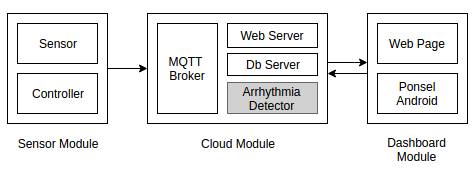
\includegraphics[scale=0.5]{images/overall.png}}
\caption{Overall Solution Design Diagram.}
\label{fig:overall_diagram}
\end{figure}

\subsection{Sensor Module}
Sensor Module dirancang hanya untuk membaca dan mangirimkan sinyal jantung, tidak ada pemrosesan berat pada modul. Hal ini ditujukan agar sensor dapat melakukan sampling dengan frekuensi yang tinggi. Selain itu, hal tersebut memungkinkan kedua jenis sensor (ECG atau PPG) dijadikan input pada modul. 

Sensor yang dirancang melakukan \textit{sampling} pada 200Hz atau 5ms/sampel. Frekuensi sampel yang tinggi ini membutuhkan protokol komunikasi yang cepat sehingga sampel tidak memenuhi buffer yang disediakan. Oleh karena itu, MQTT dipilih sebagai protokol komunikasi pada arsitektur yang dirancang. Setiap pesan dikirim menggunakan skema fire-and-forget pada MQTT (MQTT-QOS 0). Namun, karena tidak ada jaminan sampel sampia pada cloud perlu dilakukan penanganan data hilang. Hal ini dilakukan dengan memberikan index pada setiap sampel yang dikirim. Index ini akan direset setiap 1000 sampel untuk meminimalkan penggunaan memori pada modul dan menekan ukuran paket yang dikirim.

\subsection{Cloud Module}
Semua pemrosesan dilakukan di \textit{cloud/server}. Cloud bekerja dengan membagi pekerjaan kepada unit unit proses. Sebuah unit proses secara khusus menangani sebuah ID sensor. Sistem membuat unit proses ketika sebuah ID sensor baru saja terhubung dan menutupnya ketika ID sensor tersebut berhenti terhubung. 

Sebuah unit proses akan memproses sampel berdasarkan index yang menyertai sampel tersebut. Ketika terdeteksi index yang hilang maka akan dilakukan penanganan data yang hilang. Index hilang terjadi ketika ada lompatan index yang diterima, misalnya proses menunggu index nomor 5 tapi yang tiba index nomor 10. Penanganan data yang dilakukan ialah menghitung kemungkinan nilai yang hilang berdasarkan garis lurus dari nilai sampel terakhir yang diterima ke nilai sampel sebelumnya (persamaan \ref{eq:line}). Nilai sampel ini, baik yang asli ataupun hasil perkiraan akan disimpan dalam database pada server.

\begin{equation}
y(n) = \dfrac{n (v_{2} - v_{1})}{d} + v_{1}
\label{eq:line}
\end{equation}

$v_{1}$ adalah nilai terakhir yang diterima, $v_{2}$ adalah nilai terbaru yang diterima, $n$ adalah jarak dari index terakhir, $d$ adalah jarak index terbaru ke terakhir. $y$ adalah nilai index $n$ yang hilang

Sampel kemudian diproses untuk dilakukan filtering, r-peak detection, dan aritmia classification. Sampel yang telah difilter akan digunakan sebagai visualisasi di dashboard. Karena frekuensi sampel yang tinggi maka sampel yang telah di filter perlu dilakukan downsample untuk bisa divisualisasikan. Nilai frekuensi downsampel yang dipilih ialah 20Hz (20 FPS) agar lebih banyak device yang mampu membuka dashboard.

\subsection{Dashboard Module}
Dashboard berfungsi sebagai penerima pesan peringatan dan modul pemantauan. Dengan menerapkan MQTT pada rancangan arsitektur, maka hubungan antara modul sensor-cloud-dashboard dapat digambarkan sebagai model subscriber dan publisher. Hal ini memungkinkan banyak dashboard untuk subscribe kepada ID sensor tertentu. Sekaligus memungkinkan dikirimnya \textit{push notification} kepada semua dashboard tersebut ketika ID yang dipantaunya mengalami serangan aritmia. Dashboard module dapat berupa ponsel android maupun halaman web.
\section{Arrhyhtmia Detector}
Telah banyak penelitian dilakukan untuk mengklasifikasikan aritmia berdasarkan sinyal ECG. Terdapat metode klasifikasi yang memanfaatkan metode kecerdasan buatan seperti \textit{support vector machine} (SVM) \cite{aritmia_svm} dan \textit{Artificial Neural Network} (ANN) \cite{aritmia_ann}, ada pula yang memanfaatkan aturan yang dibuat oleh dokter ahli jantung \cite{tsipouras}. Pada arsitektur yang dirancang diterapkan klasifikasi yang memanfaatkan aturan yang dibuat oleh ahli jantung. Aturan ini pertama kali diusulkan oleh Tsipouras et al, pada percobaan mereka menghasilkan akurasi yang cukup tinggi dibandingkan dengan algoritma yang lebih kompleks \cite{tsipouras}.

Algoritma Arrhyhtmia Detector berjalan pada server (lihat gambar \ref{fig:overall_diagram}, diberi warna abu). Arrhyhtmia detector terbagi menjadi 2 tahap yaitu R-Peak detection dan Arrhyhtmia detection. R peak detection bertujuan untuk menemukan gelombang R pada sinyal ECG. Lalu R peak ini akan menjadi inputan pada Arrhyhtmia detection.

\subsection{R Peak Detection}
Deteksi puncak R dilakukan dengan memanfaatkan metode yang diajukan oleh Pan-Tomkins. Metode PanTomkins yang diterapkan dimulai dari Band Pass filtering, Derived filter, Squaring, dan Moving Window Integrator \cite{pantom}. Tahapan tersebut dilakukan untuk melakukan preprocessing terhadap sinyal jantung yang masuk (gambar \ref{fig:preprocessing}). Setelah itu PanTompkins menerapkan processing berupa adaptive thresholding terhadap sebuah window sinyal yang berukuran kecil (0.3s) \cite{pantom}. Pada window tersebut, akan dicari peak yang melewati threshold yang telah ditentukan, kemudian nilai peak akan menjadi input untuk  mengupdate nilai threshold. Ketika sekian waktu terlampaui tanpa ditemukannya peak maka harus dilakukan search back hingga posisi R terakhir yang ditemukan (gambar \ref{fig:processing_ori}).

\begin{figure}[htbp]
\centerline{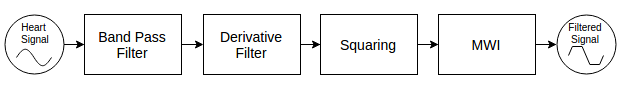
\includegraphics[scale=0.4]{images/preprocessing.png}}
\caption{Preprocessing: Filtering}
\label{fig:preprocessing}
\end{figure}

\begin{figure}[htbp]
\centerline{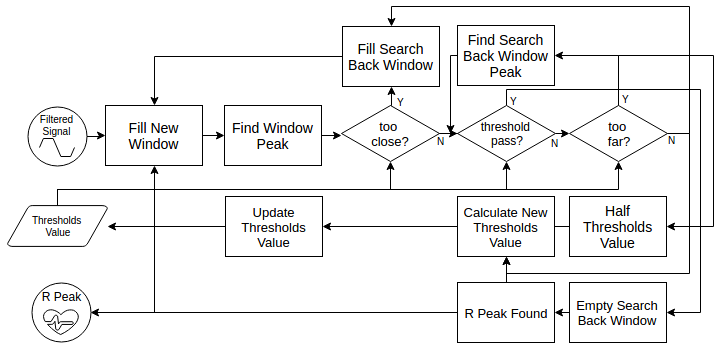
\includegraphics[scale=0.35]{images/processing_ori.png}}
\caption{Processing: Original R Peak Detection}
\label{fig:processing_ori}
\end{figure}

Penulis melihat algoritma ini dapat dioptimasi sehingga dapat bekerja lebih cepat. Optimasi dilakukan dengan mempebesar window sehingga mengurangi jumlah eksekusi yang perlu dilakukan dalam waktu yang sama, membuat threshold berdasarkan nilai rata-rata window tersebut, menghapus false beat dengan menolak R yang terlalu dekat berdasarkan rata rata jarak R (gambar \ref{fig:processing_modif}). Pelebaran window berakibat pada meningkatnya delay atas munculnya hasil deteksi sejak diterimanya sampel namun dapat meningkatkan akurasi deteksi.

\begin{figure}[htbp]
\centerline{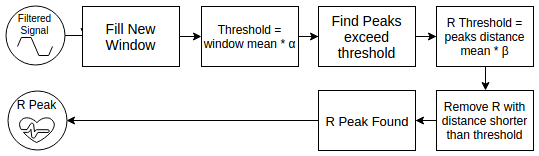
\includegraphics[scale=0.45]{images/processing_modif.png}}
\caption{Processing: Original R Peak Detection}
\label{fig:processing_modif}
\end{figure}

Nilai $\alpha$, $\beta$ serta lebar window yang diterapkan pada algoritma modifikasi didapatkan melalui hasil percobaan.

\subsection{Arrhyhtmia Detection}
Tsipouras et al. mengusulkan algoritma deteksi setelah melakukan percobaan bersama dokter spesialis jantung \cite{tsipouras}. Jenis aritmia yang dapat dideteksinya dibagi menjadi 4 jenis detak aritmia dan 7 jenis ritme aritmia. Namun untuk rancangan pada paper ini artimia hanya yang dapat dideteksi hanyalah jenis aritmia detak dan dikelompokkan kedalam 3 kategori. Kategori yang dipilih ialah 1) Normal, 2) Premature Contraction, dan 3) Ventricular Flutter. Secara detil pengelompokan ini dapat dilihat pada tabel \ref{table:beat_classification}.

\begin{table}[htbp]
	\begin{center}
	\caption{Arrhyhtmia Beat Classification}
	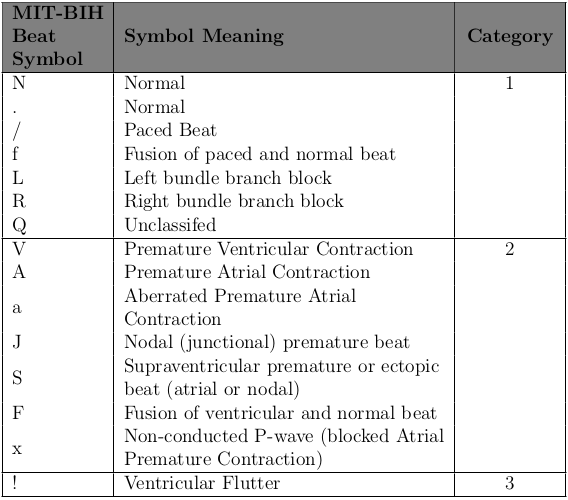
\includegraphics[scale=0.35]{images/class.png}	
	\label{table:beat_classification}
	\end{center}
\end{table}

Algoritma Tsipouras melakukan klasifikasi berdasarkan sebuah window RR interval yaitu $RR1_i$, $RR2_i$, dan $RR3_i$ yang kemudian seterusnya bergeser satu beat. Tiap beat mulanya dikategorikan sebagai kelas 1 dan kemudian mendapatkan kategori baru sesuai aturan yang telah ditetapkan (gambar \ref{fig:flowchart_aritmia}).

Rule 1. VF: Dimulai ketika $RR1_i > 1.8RR2_i$ dan durasi $RR2_i$ lebih kecil daripada 0.6 s. Maka $RR2_i$ dianggap sebagai awal mula terjandinya VF dan window berikutnya akan dites dengan kedua kondisi berikut:

\begin{enumerate}
	\item durasi setiap RR interval dalam satu window lebih kecil dari 0.7s
	\item jumlah durasi setiap RR interval dalam satu window lebih kecil dari 1.7s
\end{enumerate}

Jika salah satu kondisi tambahan pada rule 1 terpenuhi minimal 4 window berurutan maka RR2 pada tiap window tersebut diklasifikasikan sebagai beat kategori 3. Jika tidak algoritma berlanjut dan window kembali ke posisi awal ditemukannya VF.

Rule 2. PVC: Detak dikategorikan sebagai PVC jika salah satu kondisi berikut terpenuhi:

\begin{enumerate}
	\item $RR1_i > 1.15RR2_i$ dan $RR3_i > 1.15RR2_i$
	\item $|RR1_i - RR2_i| < 0.3s$ dan $RR1_i < 0.8s$ dan $RR2_i < 0.8s$ dan $1.2(RR1_i + RR2_i)/2 < RR3_i$
	\item $|RR2_i$ - $RR3_i| < 0.3s$ dan $RR2_i < 0.8s$ dan $RR3_i < 0.8s$ dan $1.2(RR2_i + RR3_i)/2 < RR1_i$
\end{enumerate}

\begin{figure}[htbp]
\centerline{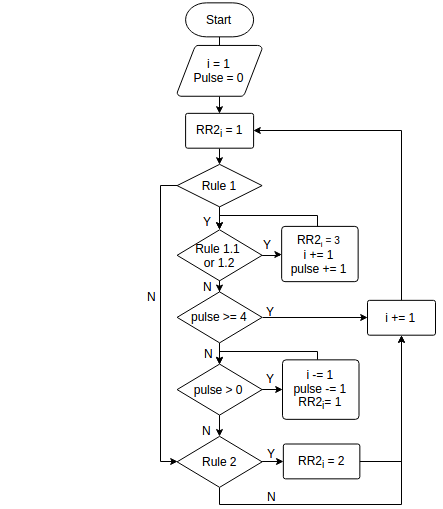
\includegraphics[scale=0.55]{images/flowchart_aritmia.png}}
\caption{Flowchart of Beat Aritmia Classification}
\label{fig:flowchart_aritmia}
\end{figure}

\section{Performance Test}
Untuk menguji performa rancangan aristektur, rancangan arsiterkur perlu untuk diterapkan. Modul sensor diterapkan menjadi bentuk gelang tangan yang ditanamkan sensor berjenis PPG. ESP-12E lalu dipilih sebagai \textit{controller}-nya. ESP-12E dipilih karena bentuknya yang kecil dan spesifikasinya yang telah memiliki modul Wi-Fi. PPG dipilih hanya untuk mensimulasikan transmisi sinyal jantung, akurasi deteksi akan diukur menggunakan dataset ECG yang telah disedikan oleh MIT-BIH \cite{mit_bih_paper, physionet}. Modul cloud diterapkan secara lokal pada komputer ASUS K432SD@2.1GHz-RAM 6GB. Cloud akan diuji menggunakan 2 buah bahasa pemograman yang populer dalam membangun sistem IoT, yaitu Node.Js dan Python yang keduanya terhubung dengan database No-SQL MongoDb. Dashboard modul diterapkan menjadi sebuah halaman web dan menjadi sebuah aplikasi pada ponsel android.

Pengujian dilakukan oleh satu orang yang mengenakan modul sensor dan bergerak secara bebas dalam daerah yang tercakup WiFi. Modul sensor, Router WiFi dan Cloud modul masih berada dalam satu wilayah yang sama sehingga diasumsikan tidak ada delay akibat proses routing. Sehingga ketika terdeteksi artimia, dashboard modul dapat segera menerima push notifikasi dari MQTT. Namun karena keterbatasan maksimum FPS yang dapat dirender oleh monitor, sampel 200Hz harus di downsample hingga 20Hz pada dashboard.

\subsection{Execution Time}
Setalah diuji, waktu eksekusi ditemukan cukup kecil. Waktu eksekusi mencakup diprosesnya sampel hingga menghasilkan deteksi aritmia (tahapan filter, save, detect). Waktu eksekusi tercatat sebesar 0.00749 ms/sampel dengan menggunakan backend Node.JS dan 0.00991 ms/sampel dengan menggunakan backend Python. Ditemukan untuk rancangan arsitektur ini penggunaan nodejs lebih baik karena dengan alogritma dan spesifikasi server yang sama node.js dapat bekerja lebih cepat hingga 13\% daripada python.

Modifikasi algoritma deteksi R juga menghasilkan performa yang diharapkan ($\alpha = 1.1; \beta = 0.8; window = 6.5s$). Modifikasi algoritma menghasilkan waktu eksekusi hingga 30\% lebih cepat dari algoritma asli PanTompkin (gambar \ref{fig:exec_time}). 

\begin{figure}[htbp]
\centerline{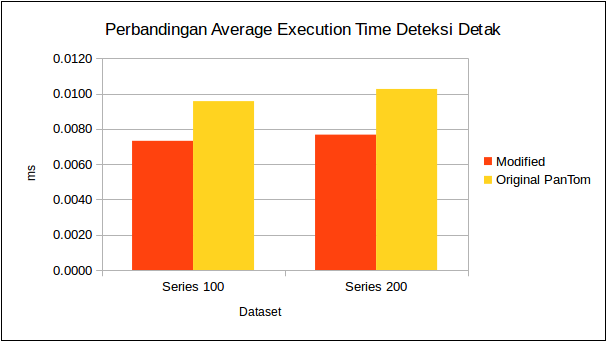
\includegraphics[scale=0.41]{images/beat_exec.png}}
\caption{Execution time comparison}
\label{fig:exec_time}
\end{figure}

\subsection{Detection}
Selain menghasilkan waktu eksekusi yang lebih cepat, modifikasi terhadap algoritma pantomkin juga memiliki tingkat akurasi yang menyamai algoritma pantomkin yang asli (gambar \ref{fig:beat_perform}). Dengan menerapkan algoritma deteksi aritmia usulan Tsipouras, sistem berhasil mendeteksi 3 kelas detak dengan performa akurasi yang cukup baik yaitu 93.11\% (gambar \ref{fig:aritmia_acc}).

\begin{figure}[htbp]
\centerline{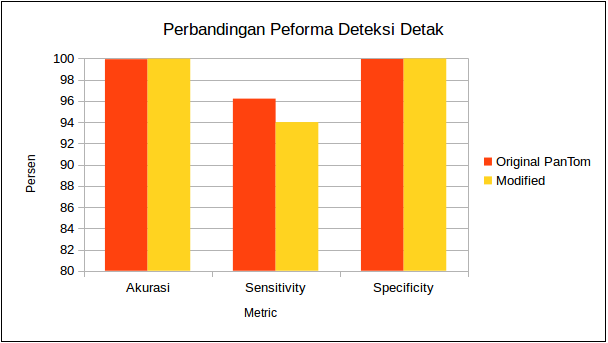
\includegraphics[scale=0.41]{images/beat_perform.png}}
\caption{Execution time comparison}
\label{fig:beat_perform}
\end{figure}

\begin{figure}[htbp]
\centerline{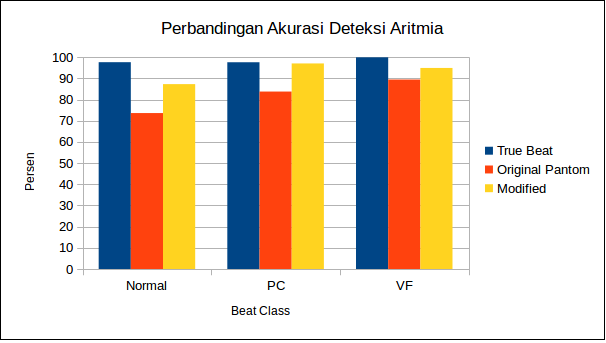
\includegraphics[scale=0.41]{images/aritmia_acc.png}}
\caption{Execution time comparison}
\label{fig:aritmia_acc}
\end{figure}

\section{Result and Conclusion}
Monitoring aritmia jantung secara realtime menggunakan IoT sangat mungkin dilakukan, terlihat dari hasil akurasi deteksi yang mencapai 93.11\%. Masalah utama berada pada optimasi resource yang terlibat, sehingga memungkinkan semakin banyak sensor dan dashboard yang dapat terhubung. Dimulai dari pemilihan bahasa server, database, hingga penerapan algoritma. Dengan menerapkan optimasi pada algoritma pantomkins server dapat menangani hingga 1.4 kali banyak sensor (waktu eksekusi berkurang hingga 30\%). Penerapan algoritma yang lebih akurat dan lebih banyak kelas yang dapat dideteksi dapat menjadi penelitian lanjutan yang menarik. \cite{huo2007short}

\printbibliography

\end{document}


